% \definecolor{color1}{RGB}{116, 184, 22}
% \definecolor{color2}{RGB}{77, 171, 247}
% \definecolor{color3}{RGB}{99, 230, 190}
% \definecolor{color4}{RGB}{132, 94, 247}
% \definecolor{color5}{RGB}{250, 176, 5}

\definecolor{color1}{RGB}{116, 184, 22}
\definecolor{color2}{RGB}{77, 171, 247}
\definecolor{color3}{RGB}{99, 230, 190}
\definecolor{color4}{RGB}{132, 94, 247}
\definecolor{color5}{RGB}{250, 176, 5}

\begin{wrapfigure}{r}{.4\textwidth}
% \vspace{-18mm}
\vspace{-5mm}
	% \begin{figure}[t] %插入图片
		\centering %图片居中
		\resizebox{.4\columnwidth}{!}{  %用于修改图片大小
			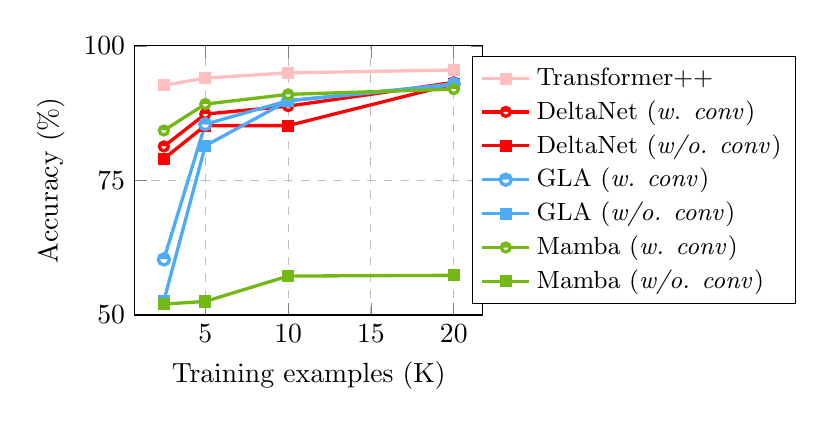
\begin{tikzpicture} %tikz图片
			\scalefont{1} %设置字体大小
			\begin{axis}[
                name=plot2,
                % at={(plot1.south east) },
			sharp plot, %控制线的风格
        title style={align=right},
        % title={Sequence Length: 512, Key-Value Pairs: 64},
			xmode=normal,% 控制坐标轴为线性
%		ymode=log,% 控制坐标轴为对数
			xlabel=Training examples (K), 
   			ylabel=Accuracy ($\%$), 
   %x坐标名
			% ylabel=y, %y坐标名
			width=6cm, height=5cm,  %设置长和宽
			% xmin=0,xmax=20,  % 设置x坐标范围
			ymin=0.5, ymax=1.0,  % 设置y坐标范围
                % x coords={1,2.5,5,10,20,40},
   			ytick={0.50,0.75,1.00}, %指定x轴刻度值。如果为空，则自动设置刻度线。即分割坐标轴,
         yticklabels={50,75,100},
			% ytick, %指定y轴刻度值。如果为空，则自动设置刻度线。即分割坐标轴
			xlabel near ticks, % 设置x坐标名位置靠近折线图
			ylabel near ticks, % 设置y坐标名位置靠近折线图
			ymajorgrids=true, % 启用/禁用 [公式] 轴上刻度线位置上的网格线
			xmajorgrids=true, % 启用/禁用 [公式] 轴上刻度线位置上的网格线
			grid style=dashed, % 设置网格线格式
			legend style={at={(1.9,0.5)},anchor=east, legend cell align=left, font=\small}, 
			]

   		\addplot[very thick, mark=square*, mark options={scale=0.8}, color=pink] plot coordinates {
% (1, 0.5453771134108428)
(2.5, 0.9266456684576904)
(5, 0.9400799353803224)
(10, 0.9497110917689993)
(20, 0.9551300417024798)
% (40, 0.9576954133935113)                    % (40, 0.9375)
% 				% (256,100)
% 				% (512,100)
			};
		\addlegendentry{Transformer++} 

   		\addplot[very thick, mark=halfcircle*, mark options={scale=0.8}, color=red] plot coordinates {
				% (1, 0.5567)
				(2.5, 0.8131)
                    (5, 0.8732)
                    (10, 0.8879)
                    (20, 0.9321)
                    % (40, 0.9375)
				% (256,100)
				% (512,100)
			};
		\addlegendentry{DeltaNet (\textit{w. conv})} 

   		\addplot[very thick, mark=square*, mark options={scale=0.8}, color=red] plot coordinates {
% (1, 0.518813082918104)
(2.5, 0.7903)
(5, 0.8518)
(10, 0.8518)
(20, 0.929)
				% (256,100)
				% (512,100)
			};
		\addlegendentry{DeltaNet (\textit{w/o. conv})} 

   		\addplot[very thick, mark=halfcircle*,  color=color2] plot coordinates {
     % (1, 0.5382)
(2.5, 0.6032)
(5, 0.8543)
(10, 0.898)
(20, 0.929)
% (40, 0.928)
};
		\addlegendentry{GLA (\textit{w. conv})} 
  
   		\addplot[very thick, mark=square*, mark options={scale=0.8}, color=color2] plot coordinates {
% (1, 0.518813082918104)
(2.5, 0.5260845398480718)
(5, 0.8142079368909123)
(10, 0.8979225872754538)
(20, 0.9273920563673214)
};
		\addlegendentry{GLA (\textit{w/o. conv})} 

  %  		\addplot[very thick, mark=circle, mark options={scale=0.8}, color=red] plot coordinates {
		% 		(1, 0.4478)
		% 		(2.5, 0.7903)
  %                   (5, 0.8518)
  %                   (10, 0.8518)
  %                   (20, 0.929)
  %                   (40, 0.926)
		% 		% (256,100)
		% 		% (512,100)
		% 	};
		% \addlegendentry{DeltaNet (\textit{w/o. conv})} 
   		\addplot[very thick,  mark=halfcircle*, mark options={scale=0.8}, color=color1] plot coordinates {
				% (1, 0.6914633107618926)
				(2.5, 0.8427092983245547)
                    (5, 0.8917725303429249)
                    (10, 0.9098144905043047)
                    (20, 0.9195555980008276)
                    % (40, 0.9166100716038952)
				% (256,100)
				% (512,100)
			};
		\addlegendentry{Mamba (\textit{w. conv})} 

   		\addplot[very thick, mark=square*, mark options={scale=0.8}, color=color1] plot coordinates {
% (1, 0.4815)
(2.5, 0.5203)
(5, 0.5252)
(10, 0.5723)
(20, 0.5737)                    % (40, 0.9166100716038952)
				% (256,100)
				% (512,100)
			};
		\addlegendentry{Mamba (\textit{w/o. conv})} 


			\end{axis}
			\end{tikzpicture}
  }
    \vspace{-6mm}
		% \caption{The x-axis is the model dimension and the y-axis is accuracy on MQAR.} 
		\caption{Accuracy (\%) on RegBench.} 
		\label{fig:regbench} 
    \vspace{-6mm}
	% \end{figure}/
\end{wrapfigure}
